\documentclass[main.tex]{subfiles}

\begin{document}
\chapter{Parallelization of DFPT calculations}

Calculations with the \texttt{PHonon} package are significantly more time intensive than \texttt{PWscf} calculations, so good parallelization is of the essence to make these calculations manageable.

\section{Optimal parallelization parameters for DFPT calculations}
The \texttt{PHonon} package offers the same three parallelization levels as the \texttt{PWscf} package, namely plane wave, k point and linear algebra parallelization.

\subsection{k point parallelization}



\begin{figure}[ht!]
    \centering
    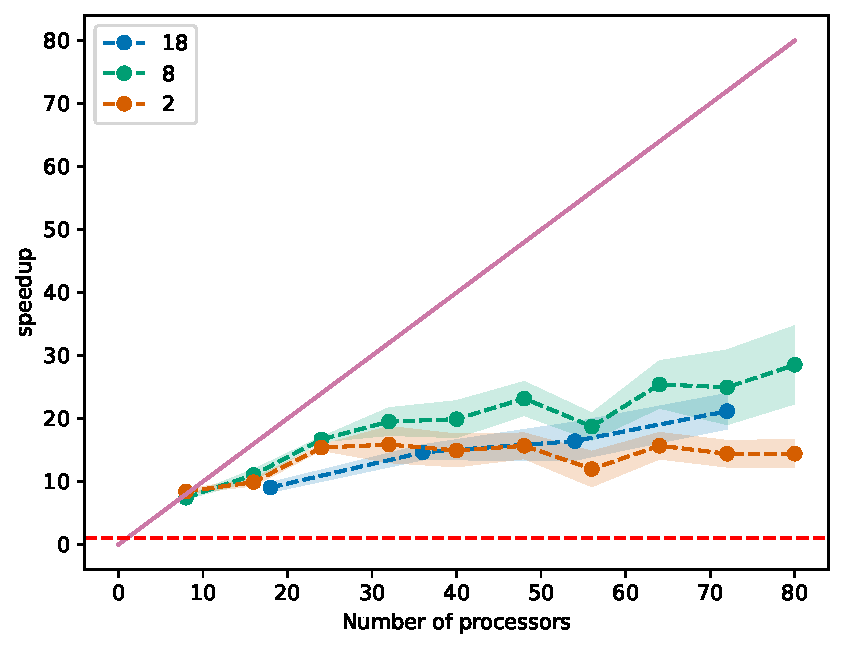
\includegraphics[width=0.8\textwidth]{plots_ph/si_ph_bench_nk_speedup.pdf}
    \caption{CAPTION}
    \label{fig:scaling_ph_nk_si}
\end{figure}

\begin{figure}[ht!]
    \centering
    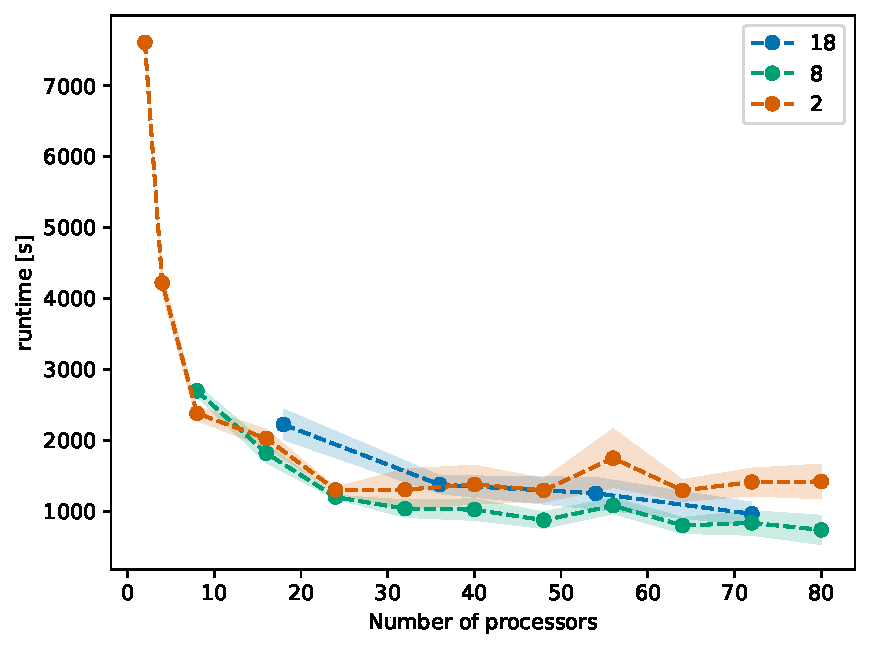
\includegraphics[width=0.8\textwidth]{plots_ph/si_ph_bench_nk_absolute.pdf}
    \caption{CAPTION}
    \label{fig:scaling_ph_nk_si_absolute}
\end{figure}

\subsection{Linear algebra parallelization}

\section{Image parallelization}

\todo{Better introduction}
When using image parallelization, \QE outputs a separate time report for every image, so one step is added to the analysis:
The total runtime of a calculation is determined by the longest running image, so speedup will be calculated using that value, but another important measure to evaluate is variation of times between images.
\begin{figure}[ht!]
    \centering
    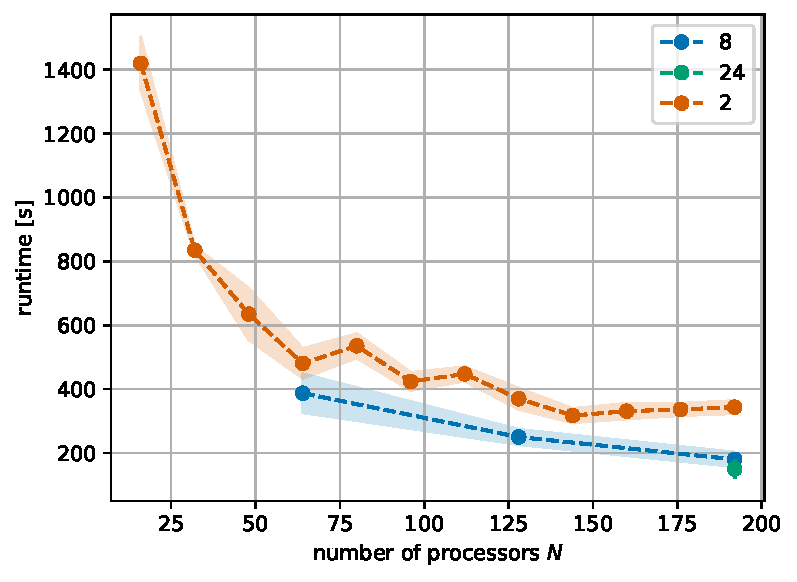
\includegraphics[width=0.8\textwidth]{plots_ph/si_ph_poolsize_8_images_distribution.pdf}
    \caption{CAPTION}
    \label{fig:scaling_ph_ni_poolsize_8_si_distribution}
\end{figure}

\begin{figure}[ht!]
    \centering
    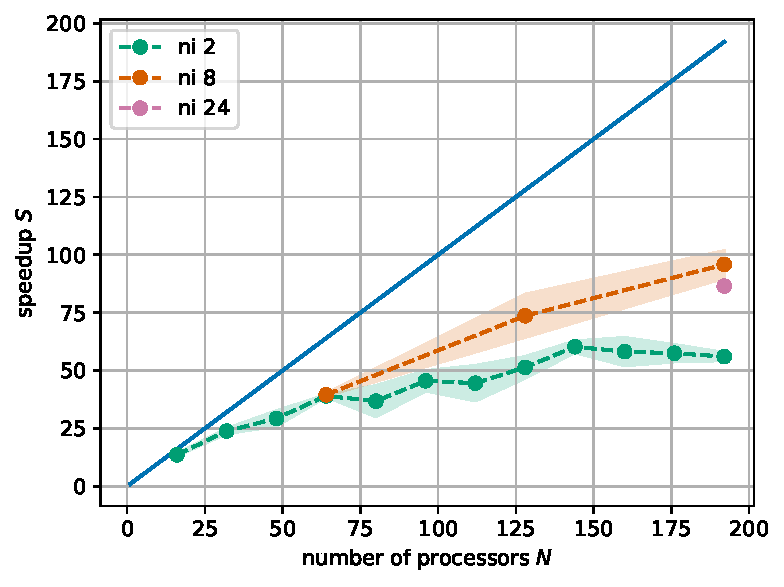
\includegraphics[width=0.8\textwidth]{plots_ph/si_ph_poolsize_8_bench_ni_speedup.pdf}
    \caption{CAPTION}
    \label{fig:scaling_ph_ni_poolsize_8_si}
\end{figure}

\begin{figure}[ht!]
    \centering
    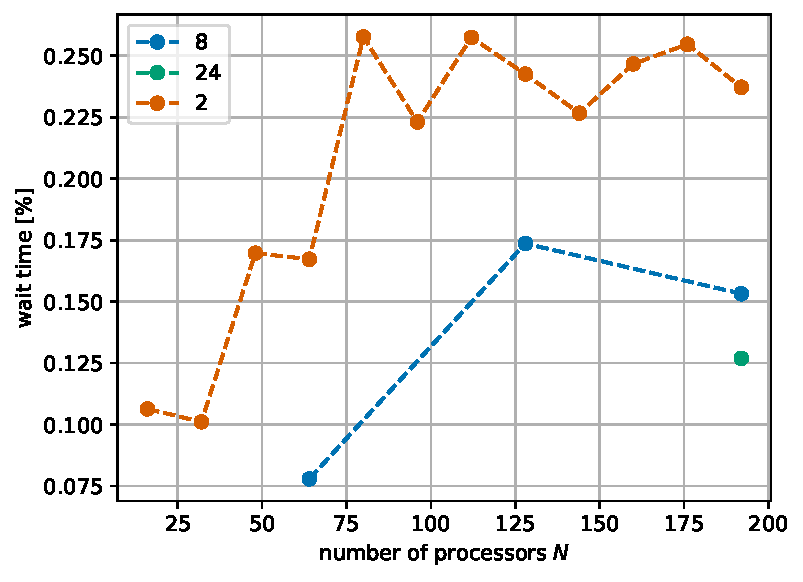
\includegraphics[width=0.8\textwidth]{plots_ph/si_ph_poolsize_8_bench_ni_wait.pdf}
    \caption{CAPTION}
    \label{fig:scaling_ph_ni_poolsize_8_si_wait}
\end{figure}

\section{Conclusion: Parameters for optimal scaling}

\end{document}